\documentclass[10pt,a4paper, oneside]{memoir}

\usepackage[utf8]{inputenc}
\usepackage[english]{babel}
\usepackage[ruled]{algorithm2e}
\newcommand*{\myalign}[2]{\multicolumn{1}{#1}{#2}}
\usepackage{listings}
\usepackage{geometry}
\geometry{a4paper, top=2cm, bottom=2cm, left= 2cm, right=2cm}
\usepackage{adjustbox}
\usepackage[english]{nomencl}
\makenomenclature
%%%%%%%%%%%%%%%%%%%%%%%%%%%%
% Chapter Style
%%%%%%%%%%%%%%%%%%%%%%%%%%%%
\usepackage{color,graphicx}
\definecolor{ared}{rgb}{.647,.129,.149}
\renewcommand\colorchapnum{\color{ared}}
\renewcommand\colorchaptitle{\color{ared}}
\chapterstyle{pedersen}
%%%%%%%%%%%%%%%%%%%%%%%%%%%%
%%%%%%%%%%%%%%%%%%%%%%%%%%%%


%%%%%%%%%%%%%%%%%%%%%%%%%%%%
%%%%%%%%%%%%%%%%%%%%%%%%%%%%
%\usepackage{calc,color}
%\newif\ifNoChapNumber
%\newcommand\Vlines{%
%\def\VL{\rule[2cm]{
%1pt}{5cm}\hspace{1mm}\relax}
%\VL\VL\VL\VL\VL\VL\VL}
%\makeatletter
%\setlength\midchapskip{0pt}
%\makechapterstyle{VZ43}{
%\renewcommand\chapternamenum{}
%\renewcommand\printchaptername{}
%\renewcommand\printchapternum{}
%\renewcommand\chapnumfont{\Huge\bfseries\centering}
%\renewcommand\chaptitlefont{\Huge\bfseries\raggedright}
%\renewcommand\printchaptertitle[1]{%
%\Vlines\hspace*{2em}%
%\begin{tabular}{@{}p{1cm} p{\textwidth3cm}}%
%\ifNoChapNumber\relax\else%
%\colorbox{black}{\color{white}%
%\makebox[.8cm]{\chapnumfont\strut \thechapter}}
%\fi
%& \chaptitlefont ##1
%\end{tabular}
%\NoChapNumberfalse
%}
%\renewcommand\printchapternonum{\NoChapNumbertrue}
%}
%\makeatother
%\chapterstyle{VZ43}
%%%%%%%%%%%%%%%%%%%%%%%%%%%%
%%%%%%%%%%%%%%%%%%%%%%%%%%%%


\title{\Huge\textbf{USER GUIDE}}
\author{\Large\textbf{M.Abdul WAHAB}}
\date{\Large{\today}}
\usepackage{color}

\definecolor{mygreen}{rgb}{0,0.6,0}
\definecolor{mygray}{rgb}{0.5,0.5,0.5}
\definecolor{mymauve}{rgb}{0.58,0,0.82}

\lstset{ %
  backgroundcolor=\color{white},   % choose the background color; you must add \usepackage{color} or \usepackage{xcolor}
  basicstyle=\footnotesize,        % the size of the fonts that are used for the code
  breakatwhitespace=false,         % sets if automatic breaks should only happen at whitespace
  breaklines=true,                 % sets automatic line breaking
  captionpos=b,                    % sets the caption-position to bottom
  commentstyle=\color{mygreen},    % comment style
  deletekeywords={...},            % if you want to delete keywords from the given language
  escapeinside={\%*}{*)},          % if you want to add LaTeX within your code
  extendedchars=true,              % lets you use non-ASCII characters; for 8-bits encodings only, does not work with UTF-8
  frame=single,	                   % adds a frame around the code
  keepspaces=true,                 % keeps spaces in text, useful for keeping indentation of code (possibly needs columns=flexible)
  keywordstyle=\color{blue},       % keyword style
  language=Octave,                 % the language of the code
  otherkeywords={*,...},           % if you want to add more keywords to the set
  numbers=left,                    % where to put the line-numbers; possible values are (none, left, right)
  numbersep=5pt,                   % how far the line-numbers are from the code
  numberstyle=\tiny\color{mygray}, % the style that is used for the line-numbers
  rulecolor=\color{black},         % if not set, the frame-color may be changed on line-breaks within not-black text (e.g. comments (green here))
  showspaces=false,                % show spaces everywhere adding particular underscores; it overrides 'showstringspaces'
  showstringspaces=false,          % underline spaces within strings only
  showtabs=false,                  % show tabs within strings adding particular underscores
  stepnumber=2,                    % the step between two line-numbers. If it's 1, each line will be numbered
  stringstyle=\color{mymauve},     % string literal style
  tabsize=2,	                   % sets default tabsize to 2 spaces
  title=\lstname                   % show the filename of files included with \lstinputlisting; also try caption instead of title
}

\begin{document}

\nomenclature{PTM}{Program Trace Macrocell: Coresight component of source class which means that PTM generates trace only if the executed instruction changed the PC (e.g. Branch instructions, load pc ..., ..)}
\nomenclature{ETM}{Embedded Trace Macrocell is a Coresight component of source class which generates trace for every executed instruction}
\nomenclature{STM}{System Trace Macrocell is a Coresight component of source class which generates trace and is the most recent component of source class}
\nomenclature{ITM}{Instrumentation Trace Macrocell is a Coresight component of source class which allows to add instructions in C code and to obtain the information that we are unable to obtain from other coresight components}
\nomenclature{Funnel}{Coresight component of link class and allows choosing which trace sources to send to the trace sinks}
\nomenclature{ETB}{Embedded Trace Buffer is a Coresight component of sink class. It is a on chip RAM allowing to store the trace generated from trace source}
\nomenclature{TPIU}{Trace Port Interface Unit is also a Coresight component of sink class and allows to send generated trace data (from trace sources) towards PL or towards outside the chip thansk to MIO}


\lstset{language=C,caption={Descriptive Caption Text},label=DescriptiveLabel}

\pagenumbering{Roman}
\maketitle
\pagebreak
\tableofcontents
\newpage
\listoffigures
\newpage
\listoftables
\newpage
\printnomenclature
\newpage
\pagenumbering{arabic}



\chapter*{Change log}
\begin{table}[]
\centering
\begin{tabular}{lccl}
\toprule
\textbf{Author} & \textbf{Version} & \textbf{Date} & \textbf{Change description}\\
\midrule
M.Abdul WAHAB & 1.0 & 18/01/2016 & 1st version (basically a draft)\\
M.Abdul WAHAB & 2.0 & 20/03/2016 & Completed Programming CS components section (\ref{sec:programming_cs_components})  \\
 & & & Change the structure of the document \\
M.Abdul WAHAB & 2.1 & 21/03/2016 & Added nomenclatures \\
M.Abdul WAHAB & 2.2 & 28/03/2017 & Changed outline and added few details in chapters \ref{chap:CS_components_Linux} and \ref{chap:overall_architecture}\\
\bottomrule
\end{tabular}
\end{table}
\pagebreak


\chapter{Introduction}
The first and the most important step of the Hardblare project is to implement DIFT (Dynamic Information Flow Tracking) also called DIFC (Dynamic Information Flow Control) on the Zedboard. Zedboard is a Xilinx Zynq SoC (System-on-Chip) which means that it contains a hardcore processor (called PS which stands for processing system) and an FPGA part (called PL which stands for programmable logic). 

\section{DIFT}
DIFT/DIFC consists of adding a tag (or label) to data of interest (e.g. inputs) and keeps track of the propagation of tags throughout the system. If any tainted data is involved in potentially illegal activity (such as pointing inside the prohibited code), an alarm is triggered. 
\subsection{Software}
Historically, the DIFT was first implemented in Software. This implementation is flexible but has the disadvantage of presenting huge overheads. For example, the least overhead while implementing DIFT in SW is 390\% which means that the program runs slower 3.9 times than the original program. This means that a better way was needed to implement DIFT on real world system.

\subsection{Hardware}
The second solution which was proposed was use hardware to implement DIFT. The main advantage of this solution is that it is quicker than the pure software solution. The disadvantages of this solution is that it is not much flexible. 

\subsection{Mix solution : SW + HW}
A third solution which was proposed was to mix the previously mentionned solutions to obtain advantages from both these solutions. Three types of solution exist in the related work. 
\begin{enumerate}
\item In-core DIFT
\item Offloading DIFT
\item Off-core 
\end{enumerate}
\vspace{1em}

In the context of this project, we will be implementing it as an off-core solution which means that the main core (or the application core) does not deal with the management of tags. The management of tags and their propagation is done on an off-core in HW. 
The main goals of this project are:
\begin{itemize}
\item Non-invasive flexible solution
\item Implement DIFT on Zedboard 
\item Low performance overhead 
\item No false positives or negatives
\item Approach based on a non-modified CPU with a standard Linux and generic binaries.
\end{itemize}
\vspace{1em}

In order to implement DIFT on zedboard, we need to obtain some informations from the CPU (PS in Zynq). Mainly these informations consist of
\begin{itemize}
\item CPU to PL 
\begin{itemize}
\item Instruction 
\item PC 
\item Memory addresses from Load and Store 
\end{itemize}
\item PL to CPU 
\begin{itemize}
\item Stall the processor
\end{itemize}
\end{itemize}

As the existing solutions implemented DIFT on the soft cores, it was easy to obtain required informations. We needed to find a way of doing this with a hard core. A solution was proposed by Master students during their project. The solution was to use the ARM debug core (called \textbf{Coresight Components}) on the ARM Cortex A9 present on the PS of Zedboard. 


\chapter{Retrieving Trace}
This chapter presents how the trace is retrieved from Coresight components. 
The chosen method is supposed to give all the informations required from CPU to PL. The proposed way is shown in figure \ref{fig:trace_retrieval}. The red box shows the PTM (Prgoram Trace Macrocell) that generates the trace and the lines in red shows the path taken by the generated trace to get to ETB (Embedded Trace Buffer) or TPIU (Trace Port Interface Unit). 

The following components belongs to the coresight components.

\begin{itemize}
\item DAP (Debug Access Port)
\item CTI (Cross Trigger Interface)
\item CTM (Cross Trigger Matrix)
\item PTM (Program Trace Macrocell) 
\item ETM (Embedded Trace Macrocell)
\item ITM (Instrumentation Trace Macrocell)
\item ETB (Embedded Trace Buffer)
\item TPIU (Trace Port Interface Unit)
\end{itemize}

These components are further divided into different categories listed in table \ref{tab:coresight_components_type}.

\begin{table}[!h]
\centering
\begin{tabular}{l|cl}
\toprule
\textbf{Type} & \textbf{Examples} & 	\textbf{Function}
\\ \midrule
Control \& Access & CTI, CTM, DAP & Give control and access to CS components \\
Sources & PTM , ETM, ITM &	collect trace from the CPU \\
Links &	FUNNEL, REPLICATOR & link between the CS sources and CS sinks\\
Sinks &	ETB, TPIU & Store or export the trace data \\
\bottomrule
\end{tabular}
\caption{Coresight Components types and function}
\label{tab:coresight_components_type}
\end{table}


\begin{figure}
\centering
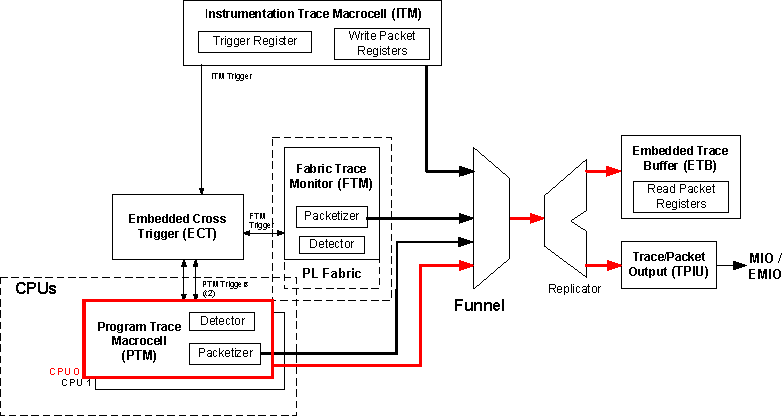
\includegraphics[width=\textwidth, keepaspectratio]{images/trace_retrieval}
\caption{Trace retrieval from ARM Cortex-A9 through Coresight Components (PTM)}
\label{fig:trace_retrieval}
\end{figure}


We need to program the CS (CoreSight) components to obtain the trace from the CPU. The trace is generated once the instruction is committed for execution (P.39/252 of PFT Architecture V1.1). Once all the components are programmed, we can start capturing the trace and decoding it in order to understand what was executed.  

\section{Programming CS components}
\label{sec:programming_cs_components}

To obtain the trace: we need to program :
\begin{enumerate}
\item Coresight source class component (PTM (on Zedboard) or it could be ETM, ITM or even STM (System Trace Macrocell) on other components)
\item Coresight link class component (Funnel)
\item Coresight sink class component (ETB, TPIU or both)
\end{enumerate}

\subsection{PTM}
To program PTM, some registers must be programmed. Beware that these registers should be programmed in a specific order as presented in figure \ref{fig:program_ptm_order}. For more information, please have a look at the c program written to program coresight components (file name is program\_coresight\_components.c and can be found on redaction\_hw gforge github). 


\begin{figure}
\centering
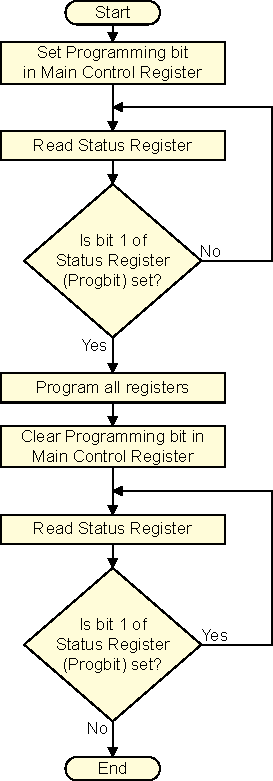
\includegraphics[width=.2\textwidth, keepaspectratio]{images/coresight/programming_ptm_registers}
\caption{PTM registers programming order}
\label{fig:program_ptm_order}
\end{figure}


The table \ref{tab:ptm_registers} presents the main registers to program in the PTM to activate it.

\begin{table}[]
	\centering
	\begin{tabular}{lcl}
	\toprule
	\textbf{Register} & \textbf{Value} & \textbf{Purpose} \\
	\midrule
	ETMLAR 	  & 	0xC5ACCE55  & 	Unlock PTM registers	\\ 
	ETMCR 	  &	1|(1<<8)|(1<<10)&	Enable PTM features	\\
	ETMTRIGGER&	0x6F			&	Events that capture trace	\\
	ETMTECR1	&	1<<24		& 	Trace all code	 	\\	
	ETMTEEVR	&	0x6F 		&	TraceEnable Event 		\\
	ETMTRACEID	&	0x0F 		& 	Trace ID 			\\
	ETMLAR 		& 	0  			& 	lock PTM registers		\\ 	
	\bottomrule
	\end{tabular}
	\caption{PTM Registers and Values}
	\label{tab:ptm_registers}
\end{table}

The following implementations for PTM are possible : 
\begin{enumerate}
\item Trace all instructions 
\item Trace range (in order to trace some functions only) or not to trace some range 
\item Trace single instruction (This feature was not implemented as it is no interest to us)
\end{enumerate}

The table \ref{tab:ptm_configuration_registers} presents the registers that need to be programmed and the bits that needs to be changed in order to program the different types of PTM implementations.

\begin{table}[]
  \centering
\begin{adjustbox}{max width=\textwidth}
\begin{tabular}{l|ccc}
\toprule
\textbf{Register} & \textbf{TRACE ALL INSTRUCTIONS} & \textbf{TRACE RANGE} & \textbf{TRACE ALL EXCEPT SOME REGIONS}\\
\midrule
ETMCR & \multicolumn{3}{c}{1 $\ll$ 10 (Change programming bit alone)} \\ 
ETMCR &  \multicolumn{3}{c}{(1 $\ll$ 8)|(1 $\ll$ 12) (Activate other features)}\\
ETMTECR1 & 1 $\ll$ 24 & 0 $\ll$ 24 & 1 $\ll$ 24 \\
ETMTEEVR & \multicolumn{3}{c}{ 0x6F (Event ALWAYS TRUE)}\\
ETMACVR(n) &  - & \multicolumn{2}{c}{Start/stop address} \\
ETMACTR(n) & \multicolumn{3}{c}{1}\\
\bottomrule
\end{tabular}
\end{adjustbox}
  \caption{PTM Configuration register}
  \label{tab:ptm_configuration_registers}
\end{table}

Here is the overview of the registers mentionned in the table \ref{tab:ptm_configuration_registers}.

 
\subsection{FUNNEL}
The funnel component is shown in figure \ref{fig:funnel} and only one register is needed to be programmed (the funnel control register shown in figure \ref{fig:cs_funnel_control_register}). In order to understand which bit to activate, we need to have a look at Zynq TRM (Technical Reference manual) which indicates which inputs are connected in the funnel. In our case, we need to activate the bit corresponding to PTM\_0 (which generates the trace of what is executer on CPU\_0). This bit is bit 0 as indicated in figure \ref{fig:cs_funnel_control_register}. The table \ref{fig:cs_funnel_control_register} resumes the register to program in descending order.


\begin{figure}
\centering
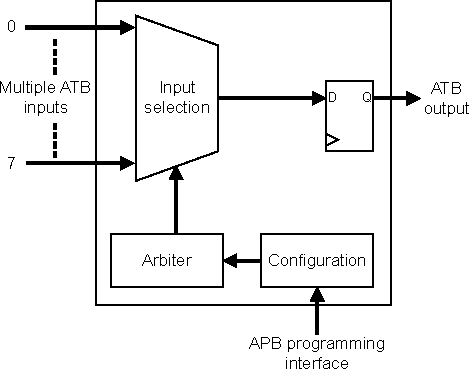
\includegraphics[scale=1, keepaspectratio]{images/coresight/cs_trace_funnel}
\caption{Coresight Funnel (Link class)}
\label{fig:funnel}
\end{figure}


\begin{figure}
\centering
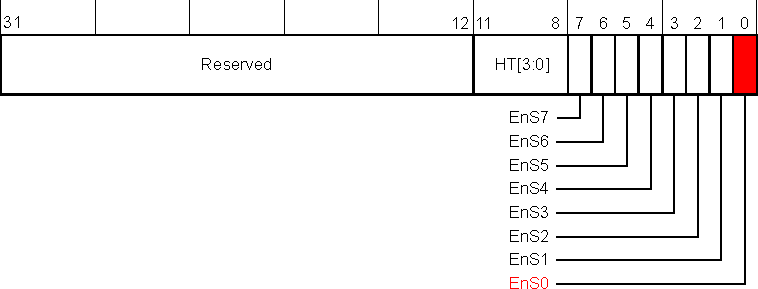
\includegraphics[scale=1, keepaspectratio]{images/coresight/cs_funnel_control_register}
\caption{Coresight Funnel (Link class)}
\label{fig:cs_funnel_control_register}
\end{figure}


\begin{table}[]
	\centering
	\begin{tabular}{lcl}
	\toprule
	\textbf{Register} & \textbf{Value} & \textbf{Purpose} \\
	\midrule
	CSTFLAR 	& 	0xC5ACCE55  	& 	Unlock FUNNEL registers\\ 
	CSTF Control	&	1			&	Enable input for trace 0 \\
	CSTFLAR 	& 	0  			& 	lock FUNNEL registers    \\ 	
	\bottomrule
	\end{tabular}
	\caption{FUNNEL Registers and Values}
	\label{tab:funnel_registers_and_values}
\end{table}


\subsection{ETB}
To program ETB, following actions need to be taken and in the presented order. The table \ref{tab:etb_register_values} shows the registers to program and the value to program with.

\begin{enumerate}
\item Program ETB registers
\item Enable tracing
\item Wait until the AcqComp bit is set
\item CODE TO TRACE GOES HERE
\item Disable tracing
\item Wait until the DFEmpty bit is set
\item Read the trace
\end{enumerate}

\begin{table}[]
	\centering
	\begin{tabular}{lcl}
	\toprule
	\textbf{Register} & \textbf{Value} & \textbf{Purpose} \\
	\midrule
	ETBLAR 	& 	0xC5ACCE55  		& 	Unlock ETB registers	\\ 
	ETBFFCR 	&	(1<<8|1<<9|1<<10)	&	Enable ETB features	\\
	ETBCONTROL&	1				&	Enable ETB Trace Capture	\\
	ETBLAR 	& 	0  				& 	lock ETB registers		\\ 	
	\bottomrule
	\end{tabular}
	\caption{ETB Registers and Values}
	\label{tab:etb_register_values}
\end{table}


\subsection{TPIU}
To activate coresight components in the Zynq under vivado processing system IP, activate trace by choosing a trace width and deciding where to connect these traces (either to EMIO or MIO). If the connection is made to EMIO (Figure \ref{fig:tpiu_trace}), it is a wire available to the PL part of ZYNQ and if the connection is made to MIO, it is available to the output ports and can be used and analysed by logic analyzers. A clock is needed by TPIU that allows to synchronize TPIU with trace analyzer. By looking at ARM Coresight Component User guide, two frequencies can be choosed (Figure \ref{fig:tpiu_trace_clk}). 

\begin{enumerate}
\item @250 MHz : data should be received only at front end
\item @125 MHz : data should be received at both ends
\end{enumerate}

\begin{figure}
\centering
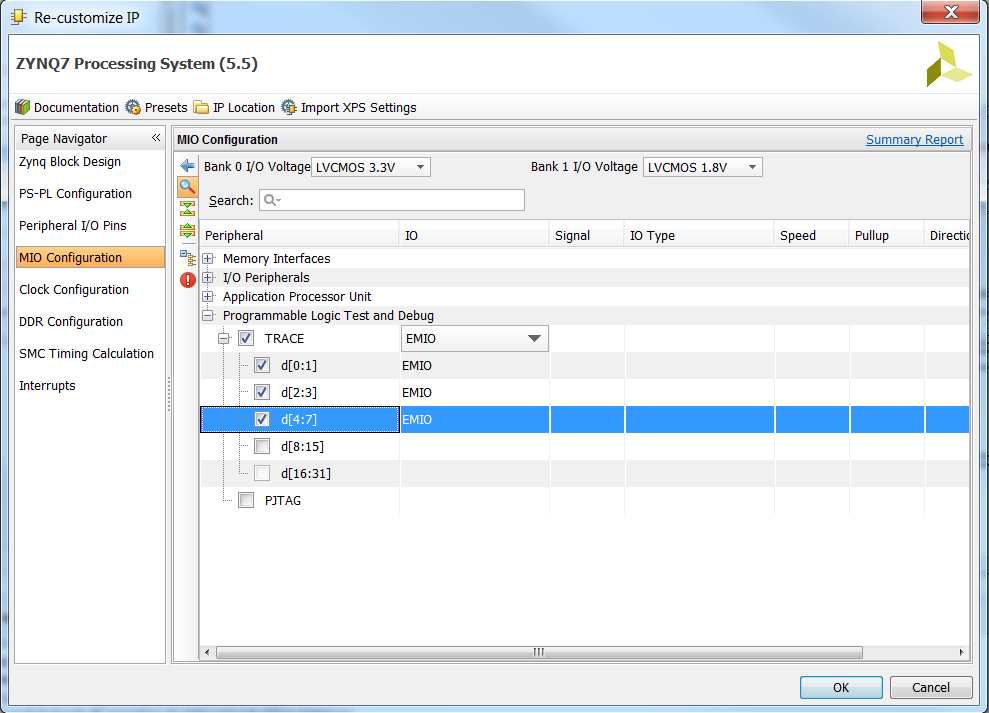
\includegraphics[scale=.6, keepaspectratio]{images/zynq_trace_tpiu}
\caption{TPIU Traces connected to EMIO}
\label{fig:tpiu_trace}
\end{figure}

\begin{figure}
\centering
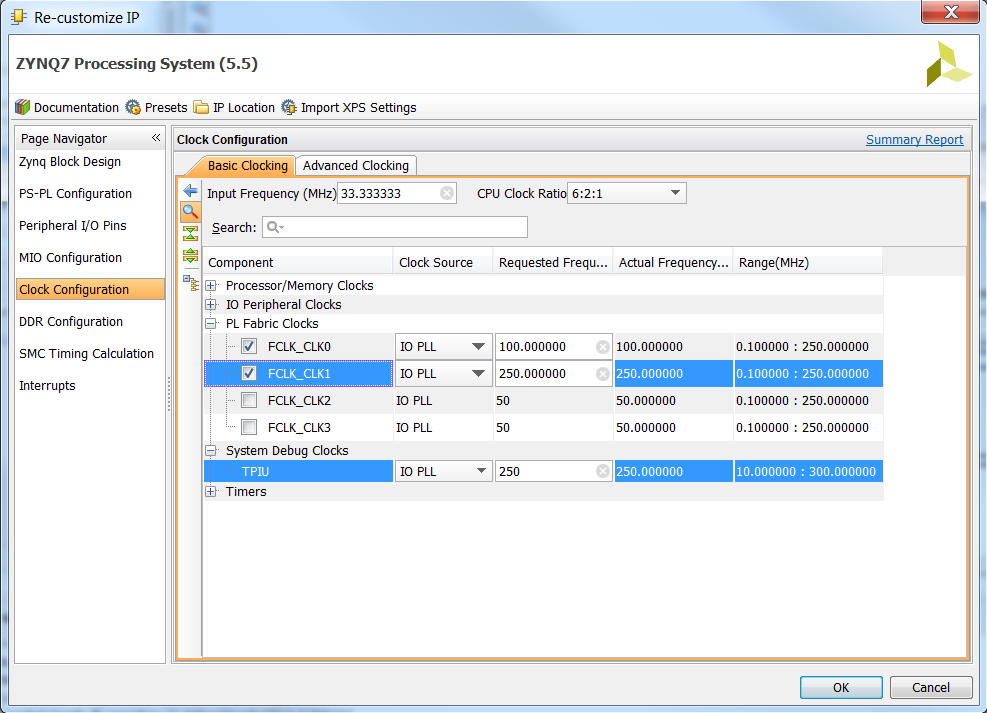
\includegraphics[scale=.6, keepaspectratio]{images/zynq_trace_clk}
\caption{TPIU Trace CLOCK}
\label{fig:tpiu_trace_clk}
\end{figure}



The frequency of 250 MHz was chosen because working with dual edge is not easy and it is not adapted to Zynq FPGA. Dual edge clock can be used in CPLD's (like Xilinx's CoolRunner II which offers the possibility of using dual edge FF's). The design realized to test if the traces collected are right is presented in Figure \ref{fig:design_test_tpiu_traces}.




\chapter{IP development}
This chapter will explain briefly some important things that we need to take into consideration when obtaining trace from the PL. These important things can be the errors I get or some important things that I read while reading a user guide. I will try to mention the source of my problem and the solution if I found one. 

\section{Goal}
The aim of IP development section is to create an IP that will allow decode obtainted PFT packets from TPIU. The decode IP should be able to decode all type of packets the PFT protocol precise. At first, the IP will be created considering single implementation of the PTM such that we know exactly the format of generated packets. 

\section{Dividing the development of IP into multiple components}
Once we programmed the TPIU, we can start getting trace on the PL. We need to store the trace sent by TPIU to PL and then decode it. We are going to need a FIFO to store the trace and to decode the trace, we will develop a custom IP in VHDL. 

\subsection{FIFO}
The best solution to implement FIFO is to use an existing FIFO\_generator IP provided by Xilinx otherwise we can replace it by a simple custom IP with following code for example. 

\subsection{PFT decoder}
To decode PFT protcol, we need to understand the PFT packets first. The table \ref{tab:pft-packets} presents the packets and their corresponding headers.

\begin{table}
\begin{tabular}{l|c|c}
\toprule
\textbf{PFT packet name} & \textbf{Header} & \textbf{Remarks}\\
\midrule
A\_sync & 0x00 00 00 00 00 00 80 & Alignment synchronization\\
I\_sync & 0x08 @@ @@ @@ @@ IB CC & Instruction synchronization\\
Atom & 0b1xxx xxx0 & \\
Branch address & 0bCxxx xxx1 & C is 1 if another byte follows, 0 otherwise.\\
Waypoint update & 0x72 & \\
Trigger & 0x0C & \\
Context ID & 0x6E & \\
VMID & 0x3C & \\
TimeStamp & 0b0100 0x10 & \\
Exception return & 0x76 & \\
Ignore & 0x66 & \\
\bottomrule
\end{tabular}
\caption{PFT packet formats}
\label{tab:pft-packets}
\end{table}

Once we know how to recognize these packets, we need to understand the order in which a packet can come. After looking at different traces we obtained so far and documentation provided by ARM on Coresight components we find out that there is no such order. This means that in almost every state, we will need to identify packet header. In order to better understand, figure \ref{} is a finite state machine describing what we want to do.

%\begin{figure}
%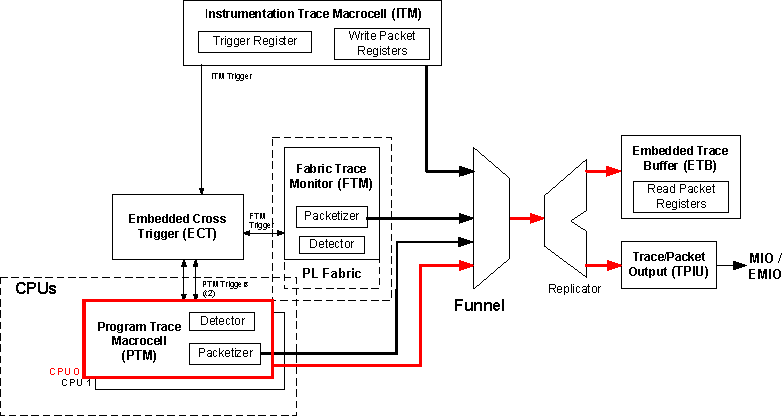
\includegraphics[width=\textwidth]{images/trace_retrieval}
%\end{figure}

\section{Timing violation problem}
To solve the timing violation problems, I tried to test each IP that I created separately to make sure if the error comes from my IP or the ones provided by Xilinx. 

\begin{itemize}
\item Vivado project name : test\_bram
\item Location : E:\textbackslash Vivado\textbackslash test\textbackslash test\_bram
\end{itemize}

The problem appears when we implement the design on the PL of zedboard. The problem stays even when we remove the nested branchs which have the consequence of making larger logic blocks. For example, the "if elsif ..." in the function was replaced by a case in order to check if it was possible to correct this implementation error without redesigning the state machine. This error was obtained regardless of synthesis and implementation strategies (Figure \ref{fig:tpiu_traces_design_runs}). 

\begin{figure}
\centering
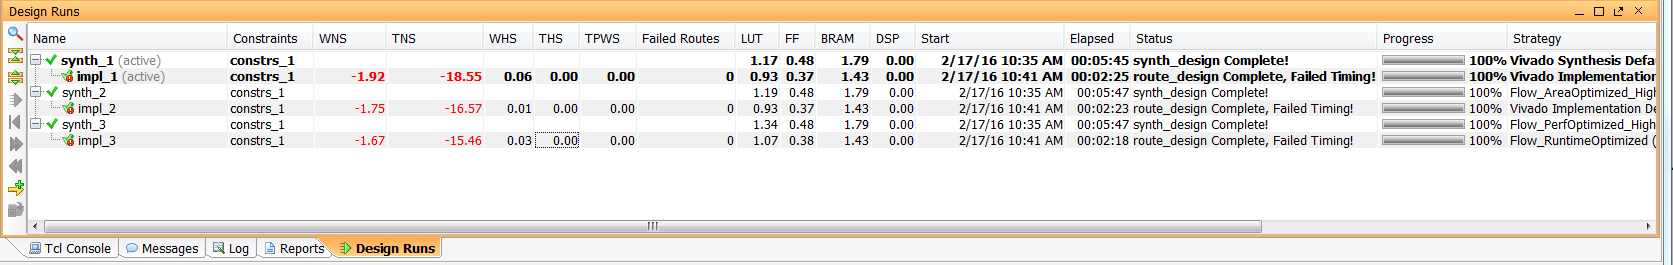
\includegraphics[scale=.5, keepaspectratio]{images/pft_decoder_timing_design_runs}
\caption{TPIU Trace CLOCK}
\label{fig:tpiu_traces_design_runs}
\end{figure}


\subsection{Mem\_Ctl}
This IP generates the signals to interface correctly to BRAM. It is not very customizable yet but it works. The design to test the IP is presented in figure \ref{fig:test_design_mem_ctl}.

\begin{itemize}
\item The mem\_ctl\_v\_1\_0 ip is located in E:\textbackslash Vivado \textbackslash test \textbackslash mem\_ctl. 
\item input data\_in value is set to constant value 0xf012340f
\item input data\_v of this IP is set to constant '1'
\item BRAM (Block Memory Generator IP) mode : BRAM controller 
\item BRAM memory type : True Dual port RAM
\end{itemize}

\begin{figure}
\centering
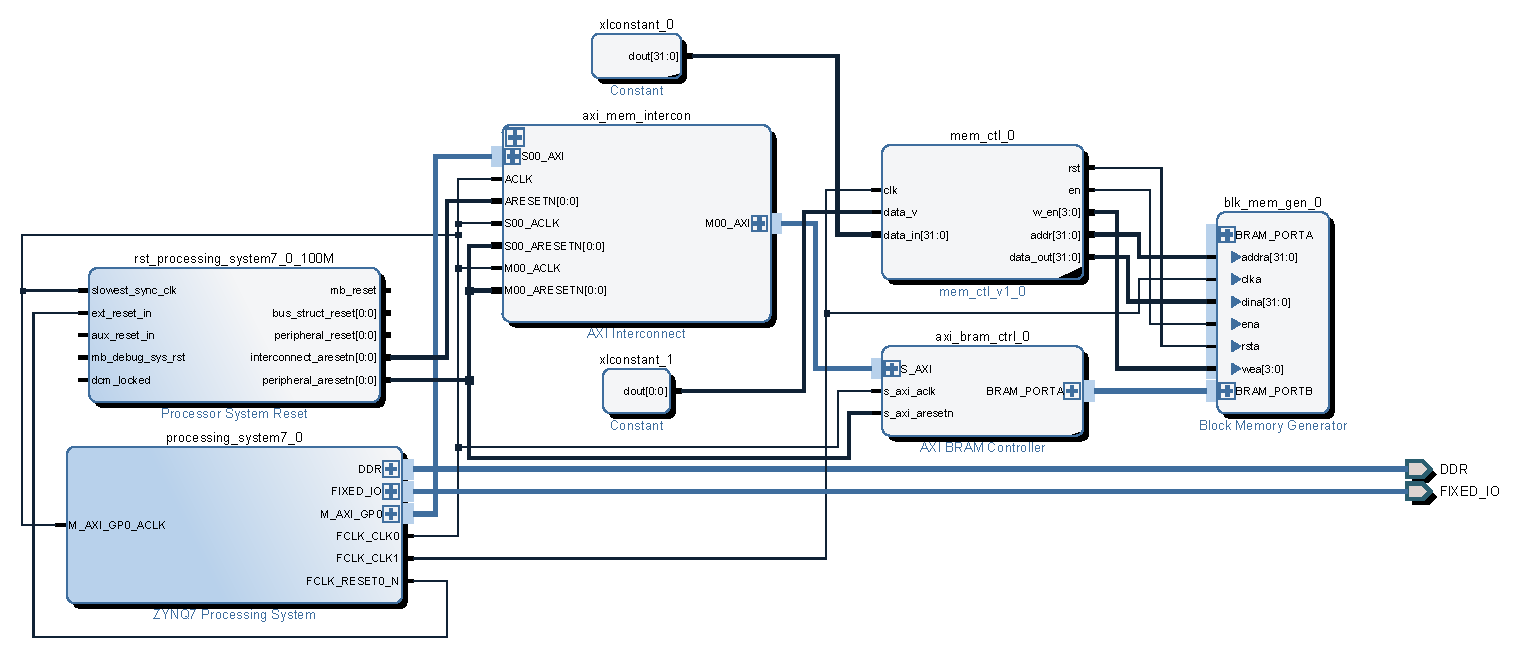
\includegraphics[scale=.6, keepaspectratio]{images/test_design_mem_ctl_bram}
\caption{Design to test BRAM}
\label{fig:test_design_mem_ctl}
\end{figure}


First, both the clocks were chosen to work at 250 MHz (because traces are generated at this frequency). Vivado default synthesis and implementation strategies were tested and it gave the "timing requirements did not meet" critical warning. 

Then, vivado synthesis settings are changed to Flow\_AreaOptimized\_High in synthesis settings (as shown in figure \ref{fig:vivado_synthesis_settings}) and Perforamce\_retiming strategy is chosen as Implementation strategy (figure \ref{fig:vivado_implementation_settings}). There was still a critical warning there. By looking at critical paths, the problem was coming from BRAM controller. It looked like the chosen frequency was too high for the BRAM Controller IP. The frequency of reads was changed to 100 MHz.

\begin{figure}
\centering
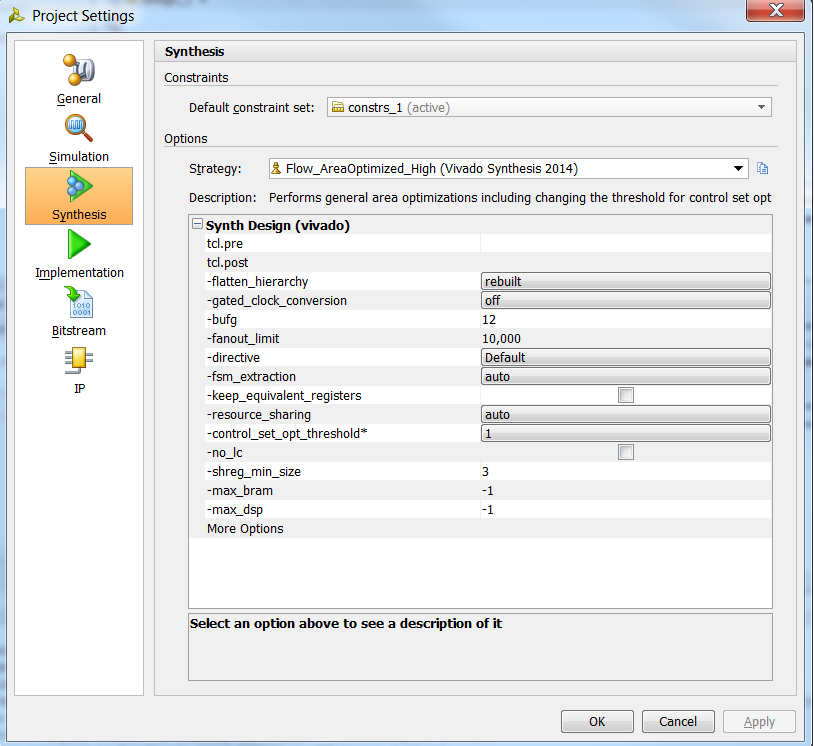
\includegraphics[scale=.4, keepaspectratio]{images/synthesis_settings_vivado}
\caption{Vivado Synthesis settings}
\label{fig:vivado_synthesis_settings}
\end{figure}

\begin{figure}
\centering
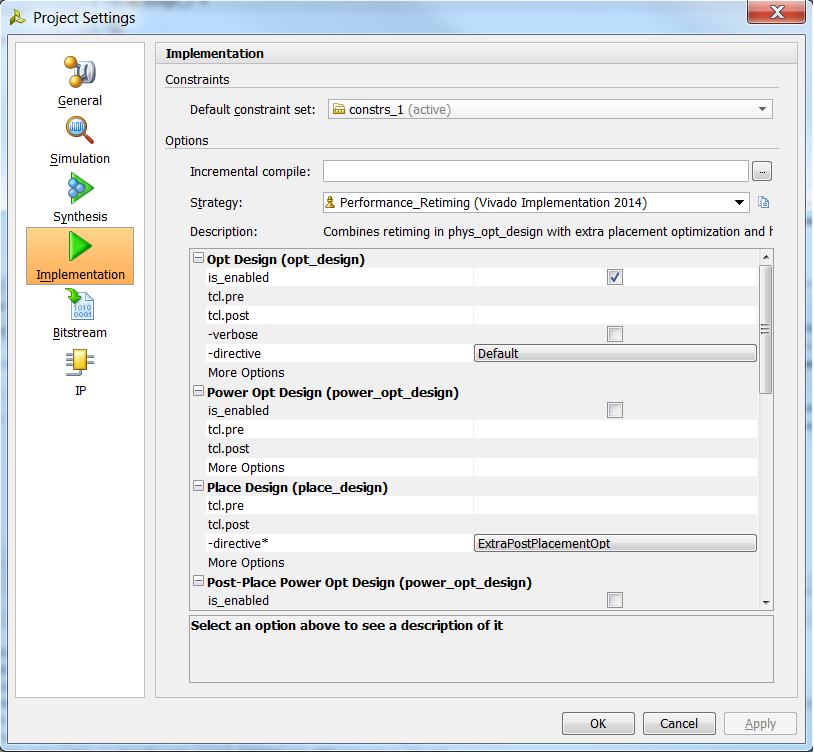
\includegraphics[scale=.4, keepaspectratio]{images/implementation_settings_vivado}
\caption{Vivado Synthesis settings}
\label{fig:vivado_implementation_settings}
\end{figure}

Then, the clock FCLK\_CLK0 is configured at 100 MHz and FCLK\_CLK1 at 250 MHz. With default synthesis and Implementation strategies, there was no critical warning on timing violation. 

The SDK project is located at E:\textbackslash Vivado\textbackslash test\textbackslash test\_bram\textbackslash test\_bram.sdk. 

An error was noticed in the generated BSP. Looking at vivado, we notice that the BRAM controller IP is mapped at address 0x40000000 (Figure \ref{fig:vivado_address_editor_mem_ctl}). On the other hand, in the generated BSP, the address was not the same (Figure \ref{fig:sdk_bsp_bram}). The XPAR\_BRAM\_0\_BASEADDR is 0x00000000 which is not the same as in the Vivado address editor which means that the defines generated by the BSP should be used carefully and checked when we use them. The C code used to read data from BRAM is presented in figure \ref{}. One strange thing to notice here is that the values read differs slightly sometimes from the original value: this may be due to cache coherency issues but needs to be taken care of once and for all.


\begin{figure}
\centering
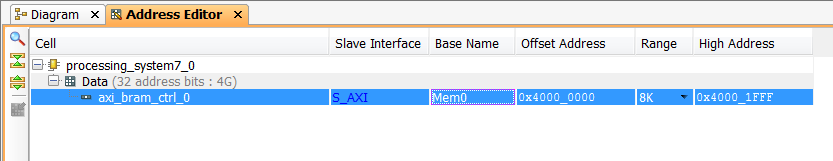
\includegraphics[scale=.4, keepaspectratio]{images/vivado_address_editor_mem_ctl}
\caption{Vivado Address editor}
\label{fig:vivado_address_editor_mem_ctl}
\end{figure}

\begin{figure}
\centering
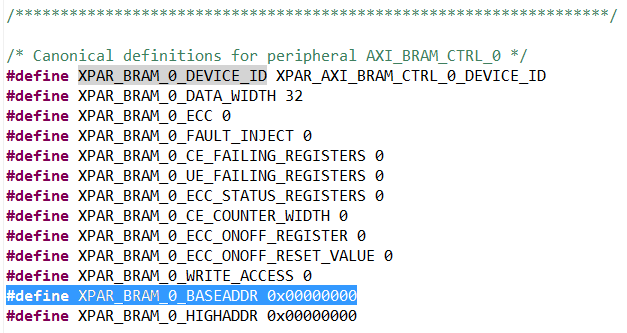
\includegraphics[scale=1, keepaspectratio]{images/sdk_bsp_bram}
\caption{Generated BSP - Xilinx SDK}
\label{fig:sdk_bsp_bram}
\end{figure}


\begin{lstlisting}
#include "xparameters.h"
#include <stdio.h>
#include "xbram.h"
#define 	BRAM_DEVICE_ID 			XPAR_BRAM_0_DEVICE_ID

XBram Bram;
int main(void)
{
	int Status, i;
	XBram_Config *ConfigPtr;

	ConfigPtr = XBram_LookupConfig(BRAM_DEVICE_ID);
	if (ConfigPtr == (XBram_Config *) NULL) {
		return XST_FAILURE;
	}

	Status = XBram_CfgInitialize(&Bram, ConfigPtr,
			ConfigPtr->CtrlBaseAddress);
	if (Status != XST_SUCCESS) {
		return XST_FAILURE;
	}

	//printf("MemBaseAddress : %08x\r\n", ConfigPtr->MemBaseAddress);

	for (i = 0; i < 200; i++)
	{
		Status = XBram_ReadReg(0x40000000, i*4);
		printf("%02x ", Status);
		if (i%20 == 0)
			printf("\r\n");
	}
	return 0;
}
\end{lstlisting}

\begin{figure}
\centering
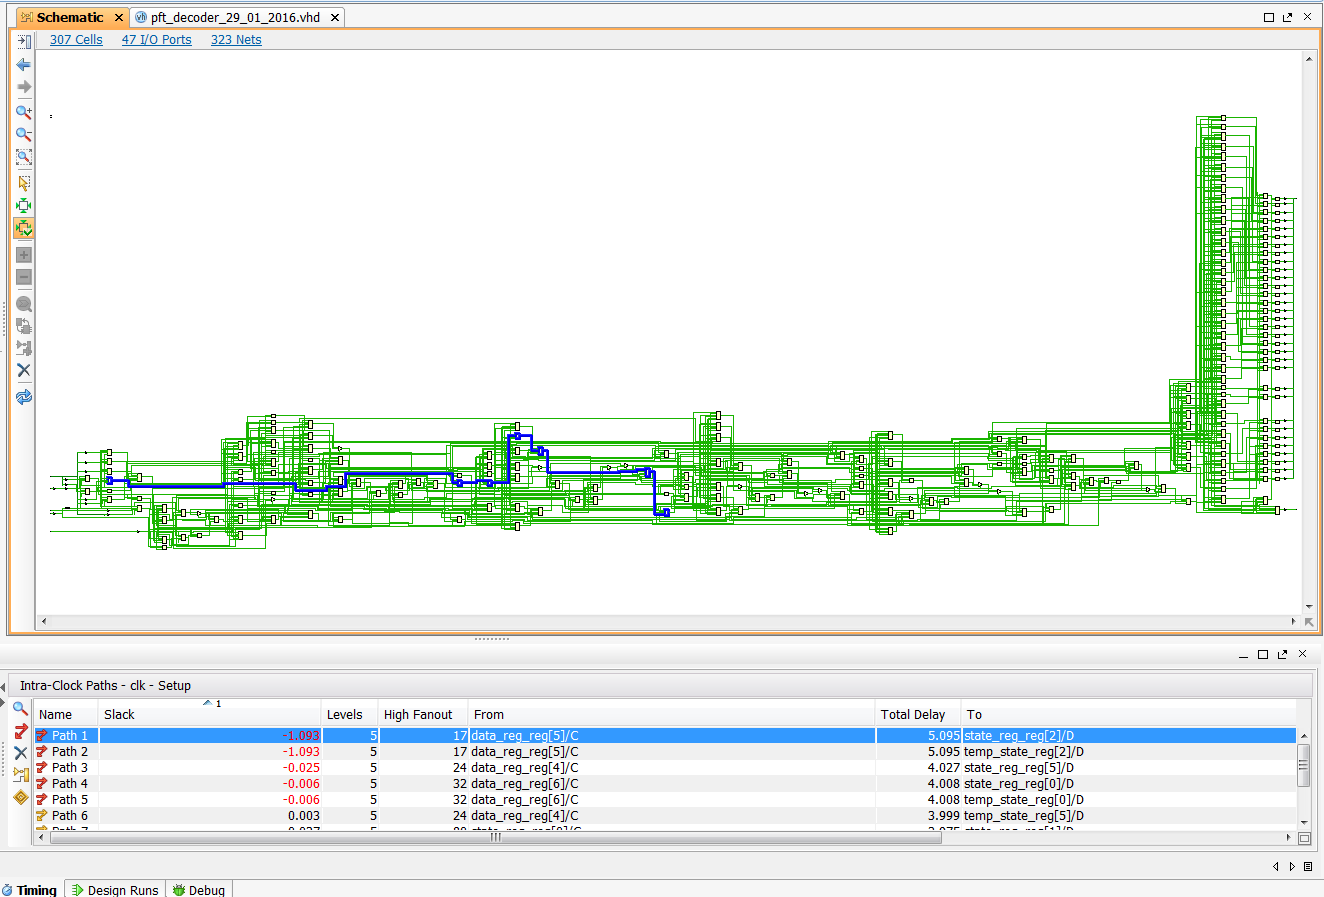
\includegraphics[scale=.6, keepaspectratio]{images/timing_violation_1}
\caption{Timing violation Path (in Blue) global design}
\label{fig:timing_violation_1}
\end{figure}


\begin{figure}
\centering
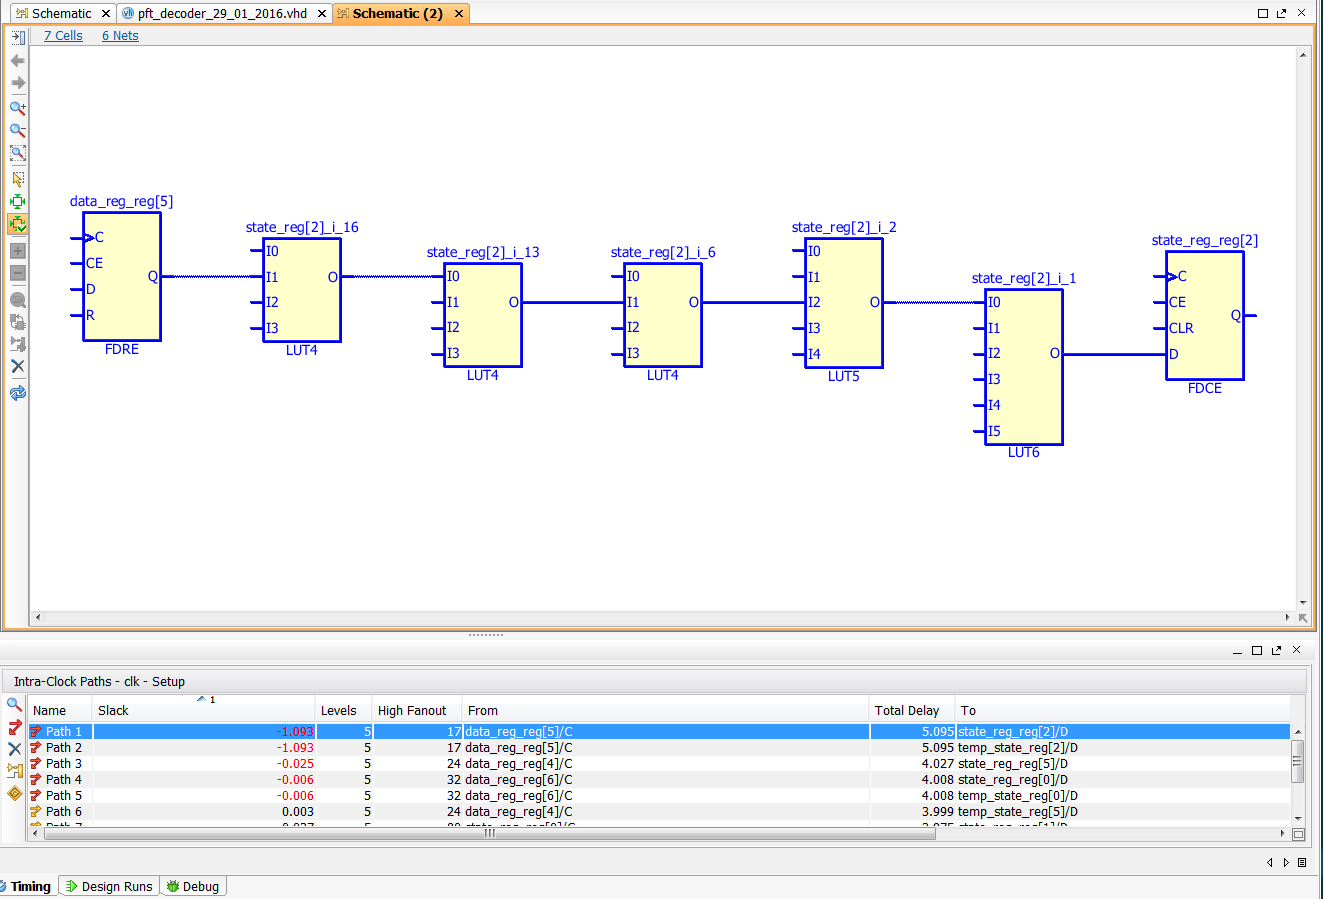
\includegraphics[scale=.6, keepaspectratio]{images/timing_violation_2}
\caption{Timing violation Path}
\label{fig:timing_violation_2}
\end{figure}


\begin{figure}
\centering
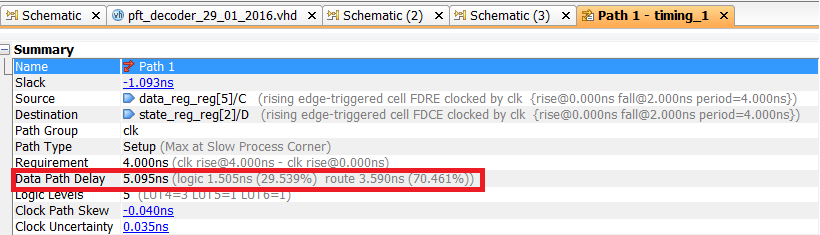
\includegraphics[scale=.8, keepaspectratio]{images/timing_violation_3}
\caption{Timing violation - Delay}
\label{fig:timing_violation_3}
\end{figure}


\section{PFT Decoder V2}
The First version of the PFT Decoder did not work although it passed every simulations (Behavioral, Post-synthesis functional, Post-implementation functional). The problem come from the fact that the FSM is too big (40-50 states) for the tool to route the design properly. If we take a look at the delays introduced by routing (See Figures \ref{fig:timing_violation_1}, \ref{fig:timing_violation_2} and \ref{fig:timing_violation_3}) it represented around 70\% of the total delay. The different things recommended by Xilinx in their FSM documentation was done in order to implement successfully the design but without any success. 

\subsection{Simple Solution}
An easy and simple solution would be to use a dual clock FIFO in which the data is written at 250 MHz and read at the maximum frequency of the decoder IP. This solution should work but this is not the right way to go before ruling out other possibilities. 

\subsection{Design smaller FSMs}
The next approach taken is to break the FSM into multiple FSMs in order to make it modular. There is one global FSM that controlls all the other FSMs. These other FSMs decode each packet: e.g. branch address packets have their own FSM which decodes the packet and so on for each packet. The packets that contains a single header are taken care of in the global FSM. 

The new design's schematic is shown in Figure \ref{fig:pft_decoder_v2_schematic}. The component chemin can be seen in figure \ref{fig:pft_decoder_v2_schematic_chemin}. The simulation showing the actual results of IP are shown in figure \ref{fig:pft_decoder_v2_simulation}. The global design realized to test the PFT Decoder v2 IP is shown in figure \ref{fig:pft_decoder_v2_global_design}. There are still few things to modify in the actual design to get an IP working at 100\%.

\begin{figure}
\centering
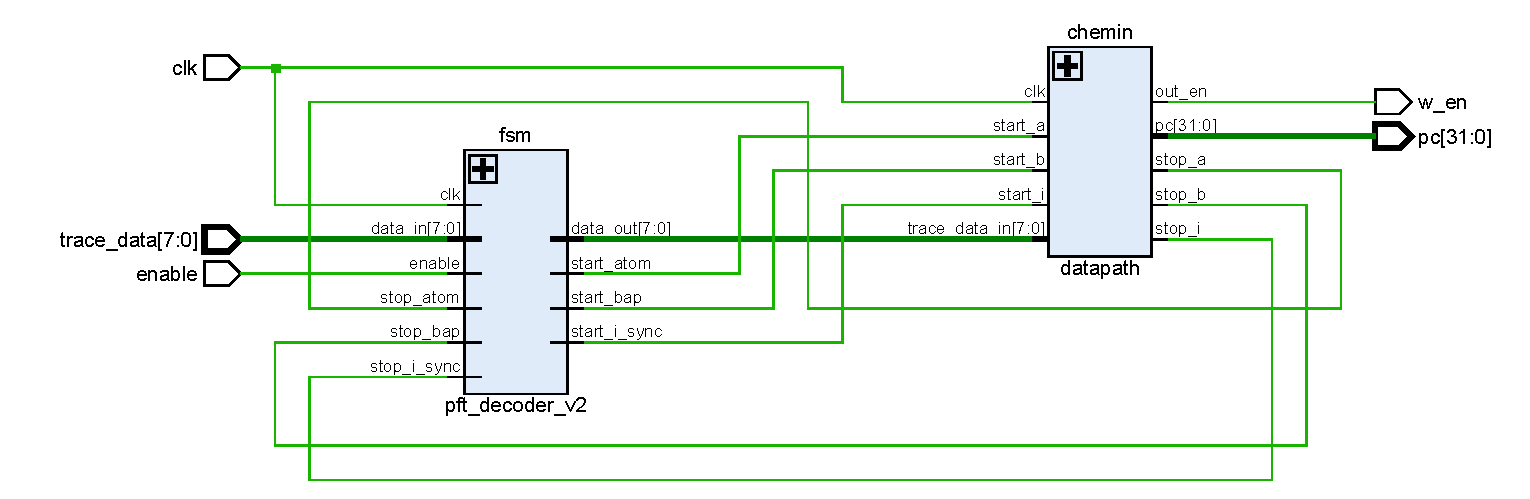
\includegraphics[scale=.7, keepaspectratio]{images/pft_decoder_v2_schematic}
\caption{PFT Decoder v2 Schematic}
\label{fig:pft_decoder_v2_schematic}
\end{figure}

\begin{figure}
\centering
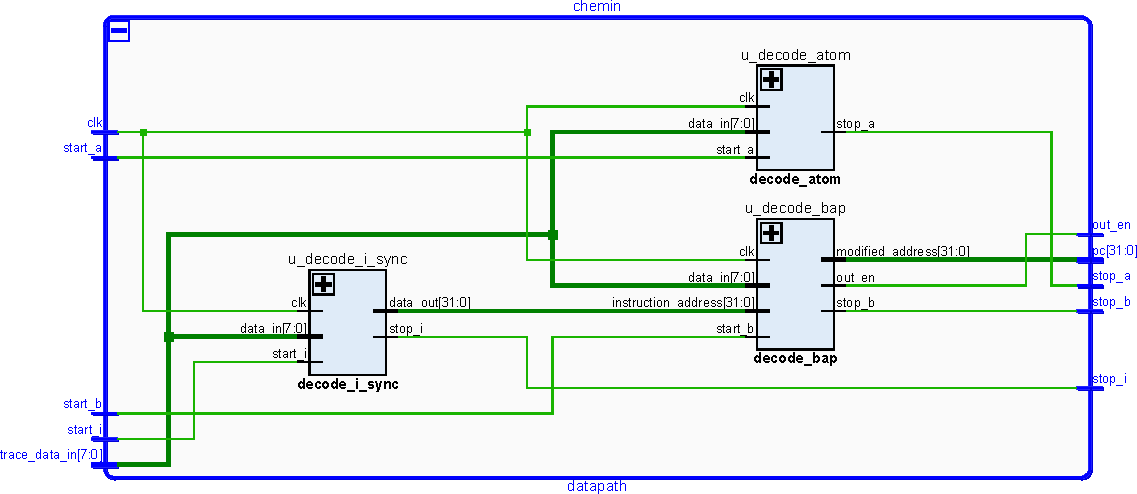
\includegraphics[scale=.85, keepaspectratio]{images/pft_decoder_v2_schematic_chemin}
\caption{PFT Decoder v2 FSMs}
\label{fig:pft_decoder_v2_schematic_chemin}
\end{figure}

\begin{figure}
\centering
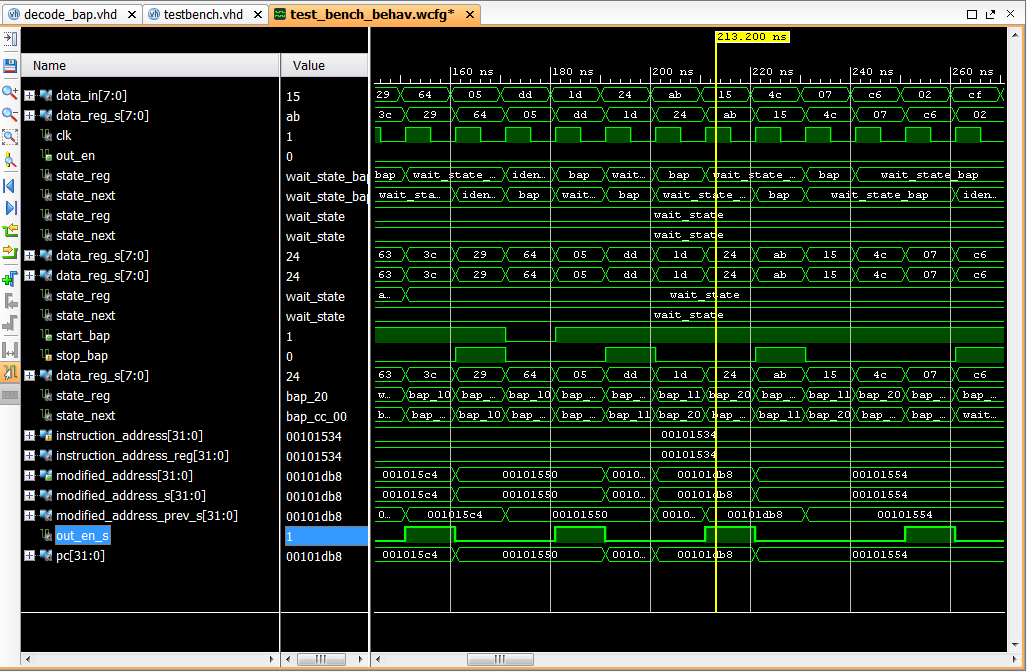
\includegraphics[scale=.8, keepaspectratio]{images/pft_decoder_v2_simulation}
\caption{PFT Decoder v2 Simulation}
\label{fig:pft_decoder_v2_simulation}
\end{figure}

\begin{figure}
\centering
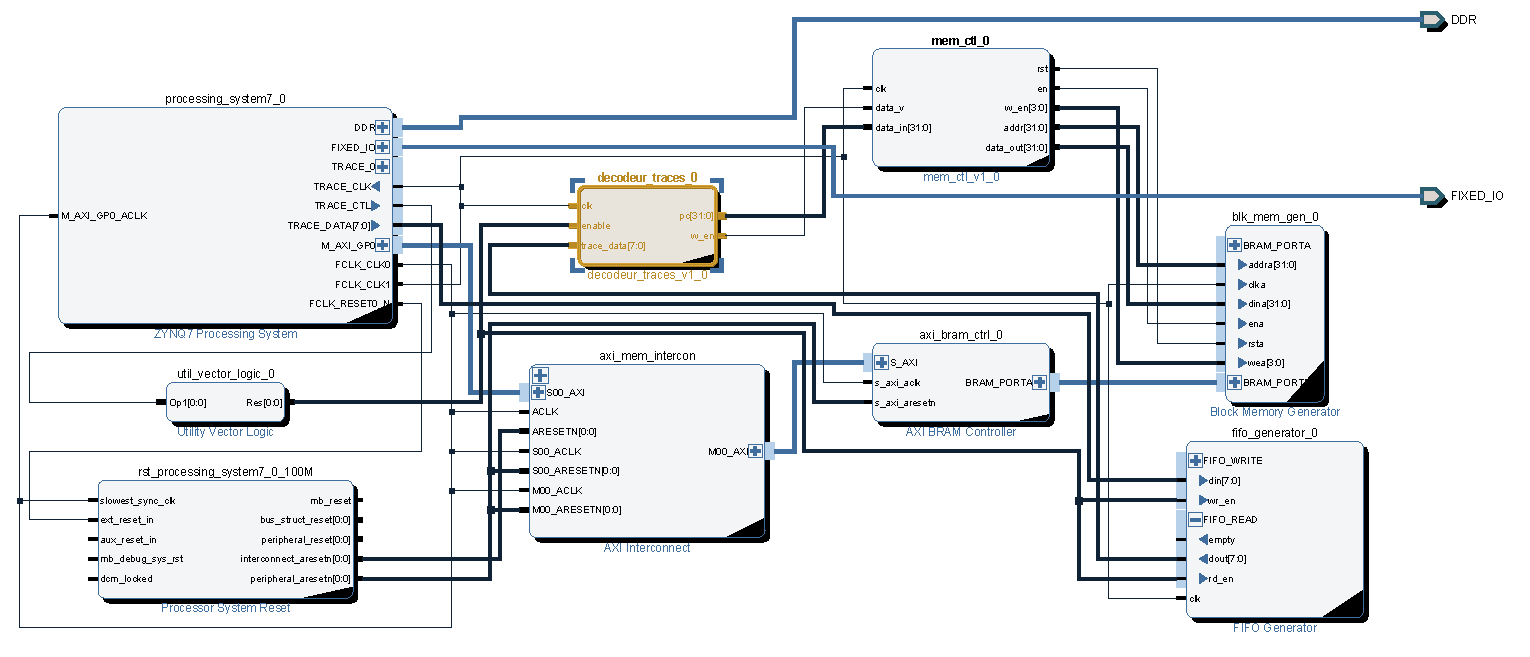
\includegraphics[scale=.74, keepaspectratio]{images/pft_decoder_v2_global_design}
\caption{PFT Decoder v2 in Global Designs}
\label{fig:pft_decoder_v2_global_design}
\end{figure}


The global design realized in order to test the Ip is presented in figure \ref{fig:tpiu_trace}.
\begin{figure}
\centering
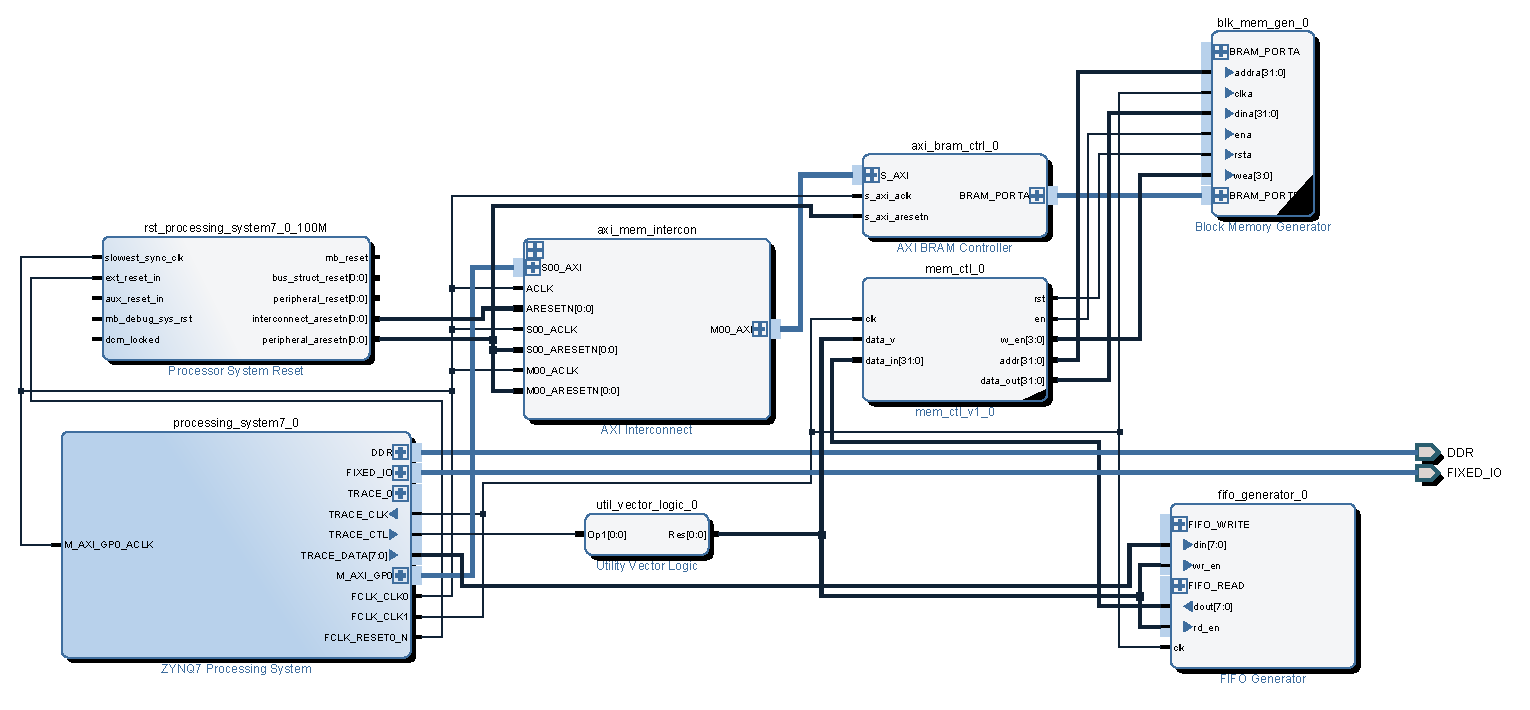
\includegraphics[scale=.6, keepaspectratio]{images/design_test_tpiu_traces}
\caption{TPIU traces PL design}
\label{fig:tpiu_trace}
\end{figure}

\begin{itemize}
\item FCLK\_CLK0 = 250 MHz
\item FCLK\_CLK1 = 125 MHz
\item BRAM Memory type : True Dual port
\item BRAM Mode : BRAM Controller
\item mem\_ctl version is located in E:\textbackslash Vivado \textbackslash test \textbackslash mem\_ctl or mem\_ctl.zip file on my personal gforge github (redaction\_hw) 
\item utility vector logic is configured to make a not gate
\item fifo generator is configured with native interface, common clock BRAM, ports write width of 8 bits
\end{itemize}



\chapter{CoreSight components in Linux}
\label{chap:CS_components_Linux}
The drivers of CoreSight components in Linux did not support our targeted device (Zynq). The first thing done was to add the support for Zynq7000 SoC. Then, the drivers needed to be modified to recover trace with expected features. Besides, we noticed that there were few problems with the TPIU driver as well. It was modified as well to recover trace in reconfigurable logic.
\section{Support for Zedboard}

\section{CoreSight PTM features}

\section{CoreSight TPIU}


\chapter{Overall architecture of first prototype}
\label{chap:overall_architecture}
\section{Design}
\subsection{First DIFT coprocessor: Microblaze}
\section{Implementation}
\subsection{First DIFT coprocessor program}
\subsection{Interrupt}
\subsection{Communication between PS (Linux) and PL}
\subsubsection{User Space}
\subsubsection{Kernel Space}
\subsection{Static analysis}
Table \ref{tab:example_trace} shows that instructions at address \texttt{860c}, \texttt{8614}, \texttt{8618}, \texttt{861c} and \texttt{8624} do not produce any trace. To recover information about all other instructions not contained in trace, the source code of program is statically analysed before execution of the program. The static analysis will generate a tag dependencies instruction that needs to be executed by DIFT coprocessor.

\begin{table}[htbp]
	%			\vspace{-\baselineskip}
	\centering
	\caption{Example tag dependencies instructions}
	\label{tab:dependencies}
	\resizebox{\linewidth}{!}{
		\begin{tabular}{|l|l|}
			\hline
			\textbf{Example Instruction} & \textbf{Tag dependencies instruction} \\ [0.2 mm]
			\texttt{sub  r0, r1, r2} & $\underline{\texttt{r0}} = \underline{\texttt{r1}}$ OR $ \underline{\texttt{r2}}$\\ [.2 mm]
			\texttt{mov  r3, r0} & 
			$\underline{\texttt{r3}} = \underline{\texttt{r0}}$\\ [.2 mm]
			\texttt{str	r1, [SP, \#4]} & $\underline{\texttt{@Mem(SP+4)}} = \underline{\texttt{r1}}$ \\ [0.2 mm]
			\texttt{ldr	r3, [SP, \#-8]} & $\underline{\texttt{r3}} = \underline{\texttt{@Mem(SP-8)}} $\\ [.2 mm]
			\texttt{str	r1, [r3, r2]} & 
			$\underline{\texttt{@Mem(r3+r2)}} = \underline{\texttt{r1}}$ \\ [0.4 mm]
			\hline
			\myalign{|c|}{\textbf{(a)}} & \myalign{c|}{\textbf{(b)}} \\
			\hline
		\end{tabular}
	}
	%			\vspace{-1.5\baselineskip}
\end{table}

If the code in Table \ref{tab:dependencies}(a) is considered, the resulting tag dependencies instruction is shown in Table \ref{tab:dependencies}(b). The tag dependencies instruction specify the operation to be realized on ARMHEx coprocessor. $\underline{\texttt{r}}$ is used to denote the tag of register \texttt{r}. For instance, for the first instruction in Table \ref{tab:dependencies}, the corresponding dependencies instruction is to associate tags of operands \texttt{r1} and \texttt{r2} towards the tag of destination register \texttt{r0}. 

%{\SetAlgoNoLine%		
\begin{algorithm}
	\SetKwInOut{Input}{Input}
	\SetKwInOut{Output}{Output}
	\Input{basic block}
	\Output{tag dependencies instructions ($tdi$)}
	\SetKwFunction{RecoverOperands}{RecoverOperands}
	\SetKwFunction{generateTDI}{generateTDI} 
	
	%	\SetKwFunction{DetermineInformationFlow}{DetermineInformationFlow}
	\SetKwFunction{isAdd}{isAdd}
	\SetKwFunction{InstructionChangesSP}{InstructionChangesSP}
	$i$ = 0;
	$operandsType$ = [];
	$operand$ = []\;
	\ForEach{instruction $instr$ in basic block}{
		
		$operandsType$[], $operand$[] = \RecoverOperands($instr$)\;	
		%	\ForEach{$operand$ in $instr$}{
		%		\Switch{operand}{
		%			\Case{reg}{
		%				$operandsType$[$i$] = $reg$\;
		%				$operand$[$i$] = $reg\_number$\;                       
		%			}	
		%			\Case{imm}{
		%				$operandsType$[$i$] = $imm$\;						
		%				$operand$[$i$] = $imm\_value$\; 
		%			}
		%			\Case{mem}{
		%				$operandsType$[$i$] = $mem$\;		
		%				$operand$[$i$] = $mem\_offset$\;  \tcp{instrumentation}				
		%			}
		%		}
		%		$i$++\;	
		%	}		
		\eIf{instr != (push OR pop OR ldm OR stm)}{
			\Switch{$\bigcup_{i}^{}$ operandsType[i]}{
				\Case{[Reg, Reg]}{
					\If{operand[1] != operand[2]}{
						$tdi$ = \underline{operand[1]} $\leftarrow$ \underline{operand[2]};}
				}	
				%				\Case{[Reg, Reg, Reg]}{
				%					\underline{operand[1]} = \underline{operand[2]} OR \underline{operand[3]};
				%				}
				\Case{[Reg, mem]}{
					$tdi$ = \underline{operand[1]} $\leftarrow$ \underline{operand[2]};
				}
				\uCase{\ldots}{}
			}
		}
		{
			\Switch{$instr$}{
				\uCase{push OR stm}{$tdi$ = \generateTDI($instr$);}	
				\uCase{pop OR ldm}{$tdi$ = \generateTDI($instr$);}
			}
		}
		\InstructionChangesSP($instr$) \tcp{Strategy 2 only}
	}
	\caption{Algorithm for generating tag dependencies instructions}
	\label{alg:static_analysis}
\end{algorithm}%		
%}
%\vspace{-\baselineskip}		
In Algorithm 1, we illustrate our algorithm that generates tag dependencies instructions. The idea is to analyze each instruction's encoding to find operands and determine information flows between these operands. The presented algorithm is applied to all basic blocks of the application to retrieve tag dependencies instructions for each basic block. These instructions are encoded and stored in a memory section. 
%{%\setlength{\interspacetitleruled}{0pt}%
%%\setlength{\algotitleheightrule}{0pt}%
%%\vspace{-.5\baselineskip}
%\begin{algorithm}
%\SetKwProg{Fn}{Function}{}{}
%\Fn{RecoverOperands}{
%	\KwIn{instruction ($instr$)}
%	\KwOut{Operands type ($operandsType$[]), \\ \hspace{1.34cm}Operands ($operand$[])}
%}	
%\Fn{generateTDI}{
%	\KwIn{instruction ($instr$)}
%	\KwOut{tag dependencies instructions ($tdi$)}
%}	
%\Fn{InstructionChangesSP}{
%	\KwIn{instruction ($instr$)}
%	\KwOut{Stack pointer offset}
%}
%\caption{Functions used by presented algorithm}	
%\end{algorithm}
%}%\vspace{-.5\baselineskip}


The \texttt{RecoverOperands} function on line 3 determines the operands for each instruction. For each operand, we determine its type (register, immediate or memory) and its value (register number, immediate value or memory address) that are stored in two lists \texttt{operandsType} and \texttt{operand} respectively. From line 4 to line 21, we determine information flows that takes place between different operands of an instruction. If an instruction has two operands and both of them are registers (case line 6), there is an information flow from the 2nd register towards the 1st register. However, if both registers are the same, there is no information flow. The conditional operation on line 7 allows to eliminate such unnecessary tag dependencies instruction. There are other cases that are not shown for simplicity. For all possible cases, we generate a tag dependencies instruction.

In ARM instruction set, most of the instructions have maximum of four operands except for some instructions. The switch case instructions from line 5 to 15 generate tag dependencies for ARM instructions that have at most four operands. However, other instructions such as \texttt{push}, \texttt{pop}, \texttt{ldm} or \texttt{stm} instructions generate multiple information flows. They need to be analyzed separately to generate tag dependencies instructions. 

The Algorithm \ref{alg:static_analysis} considers only instructions that are part of ARM instruction set. The same algorithm applies to Thumb instruction set as well but minor differences exist and are not explained here to simplify. Furthermore, the presented algorithm works for architecture ARM v7-A. It can be easily adapted to any other ARM architecture by taking into consideration minor differences that exist between instruction sets.

%For each instruction in basic block, the operands are recovered using \texttt{RecoverOperands} function. Then, the information flows can be determined using the instruction and type of operands. 
%
%To extract operands from an instruction, this function requires all ARM instructions encoding. This function returns the type of operands (\texttt{operandsType[]}), operands value (\texttt{op[]}) and number of operands (\texttt{operandsNumber}) in the instruction. 


%\begin{algorithm}
%	\SetKwProg{Fn}{Function}{}{}
%	\SetKwFunction{isAdd}{isAdd}
%	\SetKwFunction{isSub}{isSub}
%	\SetKwFunction{isLoad}{isLoad}
%	\SetKwFunction{isStore}{isStore}
%	\Fn{InstructionChangesSP($instr$)}{
%		$count$ = 0\;				
%		\Switch{instr}{
%			\Case{Reg}{
%				\If{(\isAdd \&\& $reg\_dst$ == $SP$)}{$SP$ = $SP$ + $offset$\;}
%				\If{(\isSub \&\& $reg\_dst$ == $SP$)}{$SP$ = $SP$ - $offset$\;}
%			}	
%			\Case{mem}{
%				\If{(\isLoad \&\& $reg\_src$ == $SP$)}{$SP$ = $SP$ + $offset$\;}
%				\If{(\isStore \&\& $reg\_src$ == $SP$)}{$SP$ = $SP$ - $offset$\;}
%				\If{\isPush}{$SP$ - $offset$\;}
%				\If{\isPop}{$SP$ + $offset$\;}
%			}
%		}				
%		\KwRet $SP$\;
%	}
%\end{algorithm}

\subsubsection{\textbf{Instrumentation}}

In table \ref{tab:dependencies}, the \texttt{ldr},\texttt{str} instructions contains memory addresses. These addresses need to be known to propagate their associated tags. There are three types of memory instructions (\texttt{ldr}, \texttt{str}, \texttt{ldm}, \texttt{stm}, \texttt{vldr}, \texttt{vstr}): (i) PC relative, (ii) SP relative and (iii) register relative. Some memory addresses cannot be recovered statically. We can define two possible strategies to recover memory addresses. 

\paragraph{Strategy 1}
For each memory address, an instruction is added, to the source code of program, that sends memory address(es) to ARMHEx coprocessor. 

\paragraph{Strategy 2}
From all memory instructions, only register relative instructions are instrumented. ARMHEx coprocessor knows the value of the PC thanks to CoreSight components. Therefore, we do not need to instrument memory instructions that are relative to \texttt{PC} register. Furthermore, during static analysis, if an instruction changes the SP value directly or indirectly, an instruction is added to keep track of SP value. This is taken care of by the function (\texttt{InstructionChangesSP}) on line 34 of Algorithm \ref{alg:static_analysis}. When the program is launched, the initial value of SP is sent to ARMHEx coprocessor which can then keep track of SP value changes thanks to instructions inserted during static analysis. 


\chapter{CFI: Preventing from ROP attacks}
\label{chap:CFI}
\section{Existing solution(s) and limitations}
\section{Our solution}
\section{Implementation results}

\chapter{Related Work}
\section{Articles read}

\subsection{Most recent and closest work}
To overcome high runtime overhead of software solutions, some related works propose to filter monitored events. In \cite{Fytraki2014}, a general filtering hardware accelerator that filters application events (e.g. instructions, system calls) to improve runtime performance. However, the average slowdown remains important (150\%). A similar work \cite{Chen2009} identifies common sources of slowdowns in software implementation and proposes a hardware technique to lower time overheads. However, the average slowdown remains important.

Dalton et al. \cite{Dalton07} presented one of the first implementations of a DIFT with hardware modifications. Their approach Raksha is implemented on a LEON3, an open-source SPARC v8 softcore processor developed by Gaisler Research \cite{Gaisler10}. Raksha adds several stages in the pipeline to compute tags: in other words, the architecture itself has been modified. As a consequence, performing DIFT with Raksha requires a custom processor which limits its adoption. Furthermore, Raksha is running at a low frequency of 20MHz while increasing gate count of 4.85\% over base LEON. The average time overhead for the most efficient implementation is about 200\%.

Flexitaint \cite{Venkataramani08} is an evolution of Raksha. Authors wanted to lower the impact of modifications on the processor pipeline. The Flexitaint accelerator is an in-order component placed at the end of the pipeline. This approach was simulated on a high-end processor, while ARMHEx mainly focuses on embedded system applications with lower requirements regarding processor performances. In terms of performance, Flexitaint shows latency overheads up to 8\% when tags propagation is enabled. Regarding in-core approaches, Davi et al. \cite{Davi15} implemented a similar approach with a proprietary architecture based on Intel Siskiyou Peak and SPARC (LEON3 processor).

In \cite{Dalton07,Venkataramani08}, both implementations required processor modifications: this is a major drawback as DIFT mechanisms would be hardly portable to other architectures. Offloading approaches suggest to export DIFT computations to another module. In this area, Nagarajan et al. \cite{Nagarajan08} propose to use a dual-core architecture where one core executes the main application and the operating system while the other is in charge of DIFT. This approach still adds up to 48\% in terms of computation time. Furthermore, this approach is obviously not a low-power solution as it requires an additional core identical to the main one. More recently, Jee et al. described ShadowReplica \cite{Jee13}: this work showed a slowdown of 20\% on Apache web server with an implementation on an Intel Xeon multicore architecture.

Offloading approaches are interesting as they nearly decouple DIFT computations from the main processor pipeline. The main drawback is that it needs another core for DIFT: in most cases, this additional core is oversized for such applications. Therefore, other works had a look at off-core DIFT implementations where tag computations are performed on a dedicated coprocessor. 

Kannan et al. \cite{Kannan09} proposed an evolution of Raksha \cite{Dalton07}. The communication between the coprocessor and the main core is done through a decoupling queue. The main core is configured to transmit information needed for DIFT to the coprocessor (the instruction tuple containing program counters, load/store memory addresses and instruction encoding). The coprocessor is also able to minimize stalls if both components do not run at the same frequency. Raksha as designed by Kannan et al. was fully implemented on a Xilinx Virtex-II FPGA using a LEON3 processor: the area ratio coprocessor/processor is around 8\%.
Deng et al. \cite{Deng10,Deng12} proposed Flexcore and Harmoni which are two approaches similar to Raksha \cite{Kannan09}. As for Raksha, it is implemented using a LEON3. Harmoni hardware extension \cite{Deng12} can be used for several security procedures; it presents time overheads of less than 15\% for DIFT. Dhawan et al. \cite{Dhawan15} implemented PUMP, a generic hardware support for metadata processing on a simple RISC processor.


\subsection{HARMONI, 2012 \cite{Deng:2012:HPA:2354410.2355153}}
Here is a brief summary of entitled "High-Performance Parallel Accelerator for Flexible and Efficient Run-time monitoring".
The architecture proposed in the article was designed to meet frequency requirements. The state of the art articles at the time did not take into consideration this aspect and this is the only article that tries to face this problem. The proposed architecture named HARMONI could work upto 1250 MHz. Furthermore the decoupled co-processor approach is chosen to realize runtime monitroing techniques mainly the following : 
\begin{enumerate}
\item DIFT
\item UMC (Uninitialized Memory Checking which consists of checking if a write has taken place into the memory location we are reading)
\item BC (memory Bound Checking)
\item RC (Reference Counting)
\end{enumerate}


Three types of tags are defined : 
\begin{enumerate}
\item Value tag (tag associated to data)
\item Location tag (tag associated to memory location)
\item Object tag (tag for highl-level objects such as structures, arrays, classes,...)
\end{enumerate}
Four types of operations are done on the tags: 
\begin{enumerate}
\item Read
\item Update 
\item Check 
\item Write-back
\end{enumerate}

A FIFO is used to forward entries (64) to the coprocessor. The entries are selected based on the opcode and includes : 
\begin{itemize}
\item opcode
\item register indexes of source and destination registers
\item the accessed memory address on a load/store 
\item pointer value for high-level object
\end{itemize}

The processor and co-processor can run in parallel because of the FIFO. The synchronization is done on system calls. 

\subsection{WHISK: An Uncore Architecture for Dynamic Information Flow tracking in Heterogeneous Embedded SoCs \cite{Porquet:2013:WUA:2555692.2555696}}
A quick research on the Internet allowed me to find another interesting article on applying DIFT in SoCs. What's interesting is the background study which shows how different things (such as tag storage, tag management) were done in previous architectures. This explains a little bit more how this was done previously. Most of the things explained were seen before in other articles before but here a summary can be found.

For example, for tag storage there are two types of schemes : coupled and decouples schemes. Coupled schemes consists of physically adding tag bits in the architecture which has the advantage of accessing atomically access both the tag and data in the instruction cycle. The main drawback is the need to modify the existing architecture to carry tag bit(s). 

The other approach for tag storage is the decoupled one which consists of storing data and tags separately. The main drawback is the fact that an association algorithm is needed to find the associated tag to the data.

MutekH is used as an operating system (never heard of it) and the implementation of the architecture is done using systemC. The proposed architecture consists of a DIFT wrapper ...



\bibliographystyle{plain}
\bibliography{bib/harmoni2012,bib/whisk2013,bib/sigproc}

\end{document}